\chapter{Evaluation Plan}
\label{ch:evaluationplan} 

The prototypes designed with approaches mentioned in the earlier chapter are evaluated as per the below experiment design guidelines. \\ \\

\section{Experiment Design}

\subsection{Number of Test Users}

The target users for evaluation are experienced software developers who have good knowledge of software development in general and used one of static analysis tool in their development process. So, if not the professional software developers at least the students pursuing a Masters degree in Computer Science. This ensures the evaluation process to be valid and authentic. There will be five users selected for evaluating the prototypes. One might be surprised about why only five users required, the reason behind that is well explained by Human-Computer Interaction researcher Dr. Jakob Nielsen with a simple formula\cite{five}. \\ \\

\[ N (1-(1- L )^n ) \]

Where \textbf{N} is the total number of usability problems exist in the given design, \textbf{L} is the proportion of usability problems discovered while testing a single user which is typically 31\% as found in his research. The below plot \ref{fig:5plot} further illustrates that after the number of users is five then the usability problems discovered does not increase much further as there would be high overlap with already found usability problems by previous users. Thereby, five users are selected for each iteration of the User Experience Design cycle to test the prototype designs. \\ \\

\begin{figure}[hbt!]
	\centering
	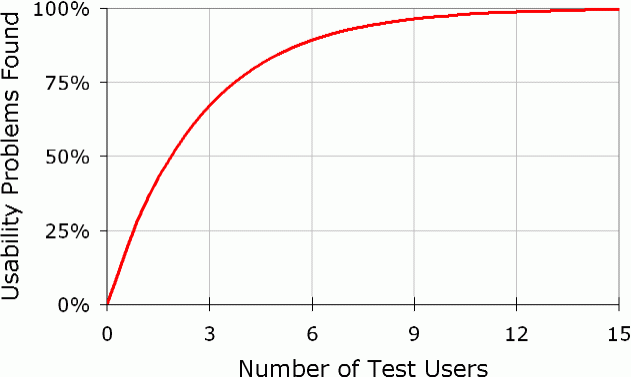
\includegraphics[width=\linewidth]{figures/fiveplot}
	\caption{A plot illustrating the usability problems found with the users.}
	\label{fig:5plot}
\end{figure}

\subsection{Order of Evaluation}

As the order of prototypes with different solution ideas presented in evaluation could influence the user as they tend to learn. Therefore, the order is changed for different segments of users which could lead to a qualitative result. For instance, let us say there are two prototypes named A and B. Half of users i..e, three in our case will have prototype A evaluated first and another half i.e., two users will evaluate B first. \\ \\

\section{Usability Inspection Methods}

There are many Usability inspection methods \cite{nielsen1994usability} like Heuristic evaluation, Heuristic estimation, Cognitive walkthrough, Pluralistic walkthrough, Feature inspection, Consistency inspection, Standards inspection and Formal usability inspection.  Out of which, the Usability aspect of the prototypes are evaluated with  'Cognitive walkthrough' and 'Heuristic evaluation'. \\ \\

\subsection{Cognitive Walkthrough}

In Cognitive walkthrough, users are asked to perform tasks with predefined steps. For each step, there are questions examined to determine usability. Blackmon, Polson, et al. in their paper \cite{blackmon2002cognitive} mentions four questions which are significant to analyse while performing Cognitive Walkthrough for the Web. They are;  \\ \\

\begin{enumerate}
	\item Will the user try and achieve the right outcome?	
	\item Will the user notice that the correct action is available to them?
	\item Will the user associate the correct action with the outcome they expect to achieve?
	\item If the correct action is performed; will the user see that progress is being made towards their intended outcome?
\end{enumerate}

These questions are also quite applicable in our context. Thereby, these questions are assessed for each step which is predetermined with designed elements on the user interface in order to solve the Research question been tackled. So, the steps vary for each design. This approach gives qualitative feedback from a user as they are a mostly open-ended scenario to discuss especially, for questions which are answered as 'No' would lead to having their suggestions/feedback. \\ \\

\subsection{Heuristic Evaluation}

In a Heuristic evaluation, the overall design is evaluated after the user has gone through the interface once or twice understanding the workflow/architecture. Then the design is evaluated with Heuristics which are called rules of thumb in the examination of usability problems. Nielsen proposed ten heuristics as standard such as, Visibility of system status, Match between system and the real world, User control and freedom, Consistency and standards, Error prevention, Recognition rather than recall, Flexibility and efficiency of use, Aesthetic and minimalist design, Help users recognize, diagnose, and recover from errors and Help and documentation. \\ \\

Once the evaluator went through the design twice, he/she mentions the problems in the context of certain heuristic. They could go through each problem mentioned with severity rating ranging from 0 to 4, where 0 - do not agree this is a usability problem, 1 - cosmetic problem, 2 - minor usability problem, 3 - major usability problem ( important to fix ), 4 - usability catastrophe ( imperative to fix ). Finally, the list of problems with severity is gathered from all evaluators. Then, the accumulated results help in re-designing the prototypes taking care that the current issues are addressed for the next iteration of the User Experience Design cycle. This evaluation process also gives valuable qualitative feedback. \\ \\

Overall, both Cognitive walkthrough and Heuristic evaluation helps to identify the usability problems in detail as possible which is qualitative analysis. Further, when more than two best solution ideas are needed to evaluated against each other then a Heuristic estimate method could be considered. It is simply to estimate which is more accepted by users with a parameter of the majority, where more number of users/evaluators could determine the stronger validity of voting which is quantitative analysis. \\ \\

\let\cleardoublepage\clearpage